%!TEX root = ../main.tex
%%%%%%%%%%%%%%%%%%%%%%%%%%%%%%%%%%
% Links:
%
% Difficulty: Companies: 
%%%%%%%%%%%%%%%%%%%%%%%%%%%%%%%%%%


%\begin{figure} \centering 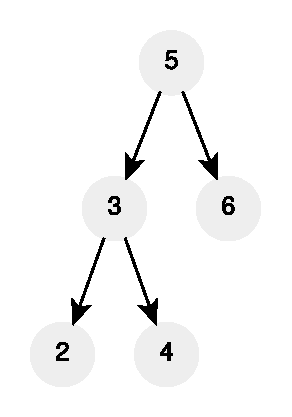
\includegraphics[width=\textwidth]{sources/max_manhattan/images/example1}
%   \caption[Sample short cpation]{Sample Caption}. \label{fig:max_manhattan:example1} \end{figure}

\chapter{Max in manhattan neighborhood$^{K}$}
\label{ch:max_manhattan}

\section*{Introduction}

This chapter discussed a very interesting problem that is based on the concept of the
\textit{Manhattan distance} \footnote{Also known as \textit{taxicab distance}.} which is as the name
suggest an alternative way to measure distances that is particularly useful in real life. Imagine
you need to measure the distance between two points on a map. You can use the old and good Euclidean
distance and come up with a number that in real life is not going to be super helpful unless you can fly. This is because that number is not going to tell you the actual distance you need to
cover if you want to get to your destination by moving on land. For instance, what is the distance
between the Empire state building and Times Square in New York? If you are not naturally equipped
with wings than all you do is to jump on a car or a cab or a bike and follow the grid pattern of
streets of Manhattan and you would have to probably cover around 15 blocks north and 3 south (See
Figure \ref{fig:max_manhattan:distance_manhattan}). The idea of measuring the distance by only
counting the number of steps we take in the north-south or west-east directions underlies what is
known as the taxicab distance. In this framework, the distance is not represented as a straight line
going from point A to point B (like it would for the Euclidean distance) but it is a zig-zagged
sequence of vertical and horizontal segments, representing movements along the north-south and
east-west axis. Therefore, the formula for measuring the taxicab distance is all about measuring
the length of the horizontal and vertical segments. The formula for measuring the manhattan distance in
Equation \ref{eq:max_manhattan:distance_formula}.
\begin{equation}
    d = |x_1-x_2|+|y_1-y_2|
    \label{eq:max_manhattan:distance_formula}
\end{equation}

The problem in this chapter will challenge you to find, for each cell of a given matrix, the largest
value in any cell sitting at a Manahtann distance below a certain threshold.

\begin{figure}
    \centering
    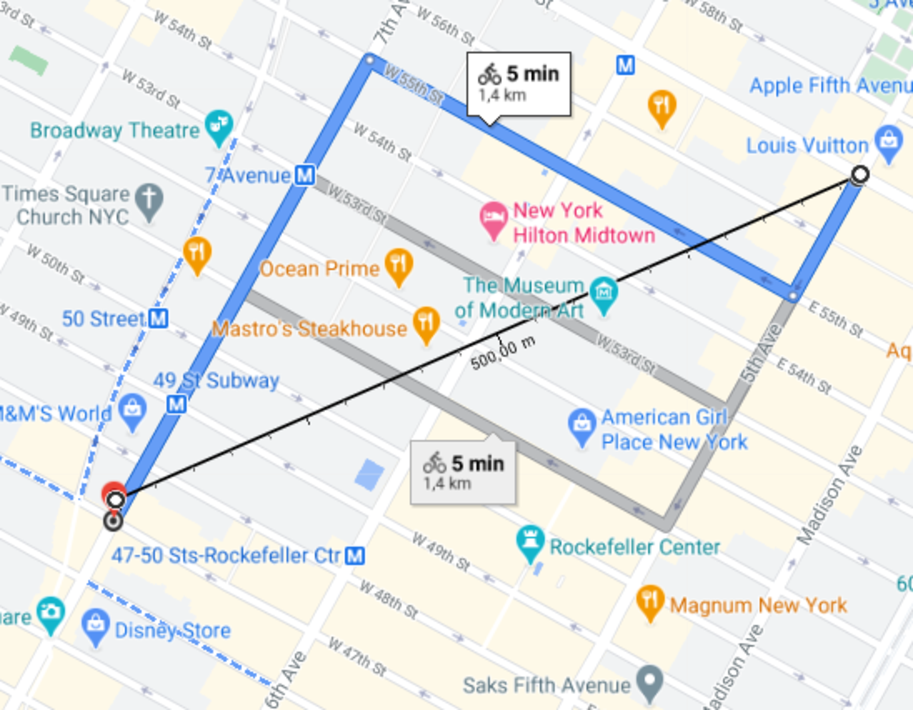
\includegraphics[width=\textwidth]{sources/max_manhattan/images/distance_manhattan2}
    \caption[Taxicab distance from times square to the trump tower]{Taxicab distance from times
    square to the Trump's tower. Notice that the black straight-line is depicting the Euclidean
    distance, and that the latter is shorter than the actual taxicab distance between  the two
    points.}
    \label{fig:max_manhattan:distance_manhattan}
\end{figure}

\section{Problem statement}
\begin{exercise}
\label{example:max_manhattan:exercice1}
Write a function that given \begin{enumerate*}
    \item a matrix $I$ of $n$ rows and $m$ columns and
    \item  an integer $K > 0$
\end{enumerate*}
returns a new matrix $M$ of size $n \times m$ where $M[i][j]$ contains the maximum value among the
elements in the manhattan neighborhood of size $K$ for the cell $(i,j)$. The Manhattan neighborhood
of size $K$ for a cell $(i,j)$ is composed of all cell $(p,q)$ such that:
\begin{equation}
    N(i,j, K) = \{(p,q) | |i-p|+|j-q| \leq K\}
    \label{eq:max_manhattan:neighbood_equation}
\end{equation}


\end{exercise}
    %example1
    \begin{example}
        \label{example:max_manhattan:example1}
        \hfill \\
        Given: $I=
        \begin{bmatrix}
          1 & 2 & 3  \\
          4 & 5 & 6  \\
          7 & 8 & 9  
        \end{bmatrix}
      $
  and $K=1$ the function return $I=
  \begin{bmatrix}
      4 & 5 & 6  \\
      7 & 8 & 9  \\
      8 & 9 & 9  
    \end{bmatrix}
$
        
    \end{example}

    %example2
    \begin{example}
        \label{example:max_manhattan:example2}
        \hfill \\
        Given: $I=
        \begin{bmatrix}
          1 & 2 & 3  \\
          4 & 5 & 6  \\
          7 & 8 & 9  
        \end{bmatrix}
      $
  and $K=2$ the function return $I=
  \begin{bmatrix}
      7 & 8 & 9  \\
      8 & 9 & 9  \\
      9 & 9 & 9  
    \end{bmatrix}
$
        
    \end{example}




\section{Clarification Questions}

\begin{QandA}
    \item 
    \begin{answered}
        \textit{}
    \end{answered}
    
\end{QandA}

\section{Discussion}
\label{max_manhattan:sec:discussion}

\subsection{Brute-force}
\label{max_manhattan:sec:bruteforce}
%You can optimize by only using N*M*2 space . see solution 2
This problem can be quite easily tackled by using a brute-force approach that is finding the answer by blindly calculating the answer for each cell as per the problem statement. 
All it is necessary to find the answer for the cell $(i,j)$ is to calculate the maximum among the cells that are at a manhattan distance of at most $K$ from it (the cells that are part of the Manhattan
neighborhood of size $K$). Therefore, the problem boils down to figuring out the neighborhood for a
given cell. Figure \ref{fig:max_manhattan:neighborhood} shown an example of such a neighborhood
where the numbers inside the cells represent the distance from the cell $(i,j)$ at the center. 
\begin{figure}
    \centering
    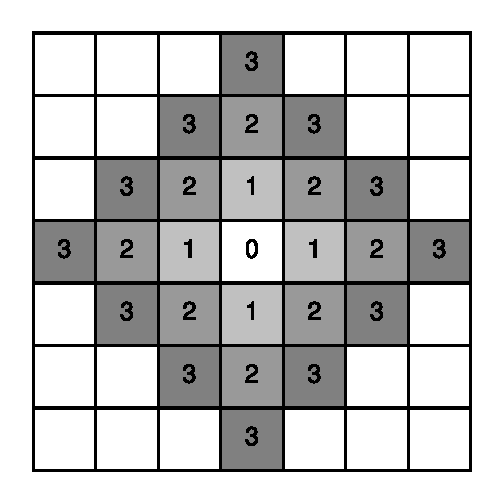
\includegraphics[width=\textwidth]{sources/max_manhattan/images/neighborhood}
    \caption[Cells in the Manhattan neighborhood of size $3$.]{Cells in the Manhattan neighborhood
    of size $3$. The numbers in each cell represent the Manhattan distance from the central cell.}
    \label{fig:max_manhattan:neighborhood}
\end{figure}
Given a cell $(i,j)$, figuring out exactly which cells are part of the neighborhood and which are
not is not particularly difficult but is definitely not trivial. Instead of coming up with a way of
generating such a list of cells, it is easier to loop over all the cells within a square of size
$2K$ having cell $(i,j)$ at its center, and to ignore the ones that do not satisfy Equation
\ref{eq:max_manhattan:neighbood_equation}. Because both 
\begin{enumerate*}
    \item the number of cells in the neighborhood and 
    \item the number of cell in such square \end{enumerate*} is quadratic in $K$, then,
asymptotically speaking, the additional work required by visiting cells that are inside the area of
cells we are looping on but not part of the neighborhood does not really make any difference.
Listing \ref{list:max_manhattan:bruteforce} shows an implementation of such idea. This approach is
clearly correct and has a time complexity of $O(nmK^2)$ as for each of the $nm$ cells of the matrix
we do exactly $K^2$ work. The space complexity is $O(1)$ as no additional space is used other than
the second matrix we must return.
\lstinputlisting[language=c++, caption={Brute Force solution to the problem of finding the max cell within the manhattan neighborhood of size $K$.},label=list:max_manhattan:bruteforce]{sources/max_manhattan/max_manhattan_solution1.cpp}


\subsection{Dynamic Programming}
\label{max_manhattan:sec:DP}
The brute-force solution works by blindly finding the solution for each cell without taking into
consideration whether we can use the information already calculated for other cells. What do I mean
by reusing and by already calculated answers for other cells? Consider the matrix shown in Figure
\ref{fig:max_manhattan:neighborhoodDP1_1} showing the neighborhood of size $1$ for the cells 
\begin{itemize*}
    \item $(x,y)$ (center)
    \item $(x+1,y)$ (right)
    \item $(x-1,y)$ (left)
    \item $(x,y-1)$ (top)
    \item $(x,y+1)$ (down)
\end{itemize*}
and Figure \ref{fig:max_manhattan:neighborhoodDP1_2} showing the neighborhood of size $2$ for the
cell $(x,y)$. Notice that the latter is composed by the union of the neighborhoods of size $1$ shown
in Figure \ref{fig:max_manhattan:neighborhoodDP1_1}. Therefore, if we know the answer for $K=1$ for
the cells 
\begin{itemize*}
    \item $(x,y)$
    \item $(x+1,y)$
    \item $(x-1,y)$
    \item $(x,y-1)$
    \item $(x,y+1)$ \end{itemize*} we can easily calculate the answer for $K=2$ for the cell $(x,y)$
without having to look at all the $12$ cells composing its  manhattan neighborhood of size $2$.



\begin{figure}
    \vspace*{-0.5in}
    %\hspace*{-0.5in}
    \centering
    
    \begin{subfigure}[t]{1.0\textwidth}
        \centering
        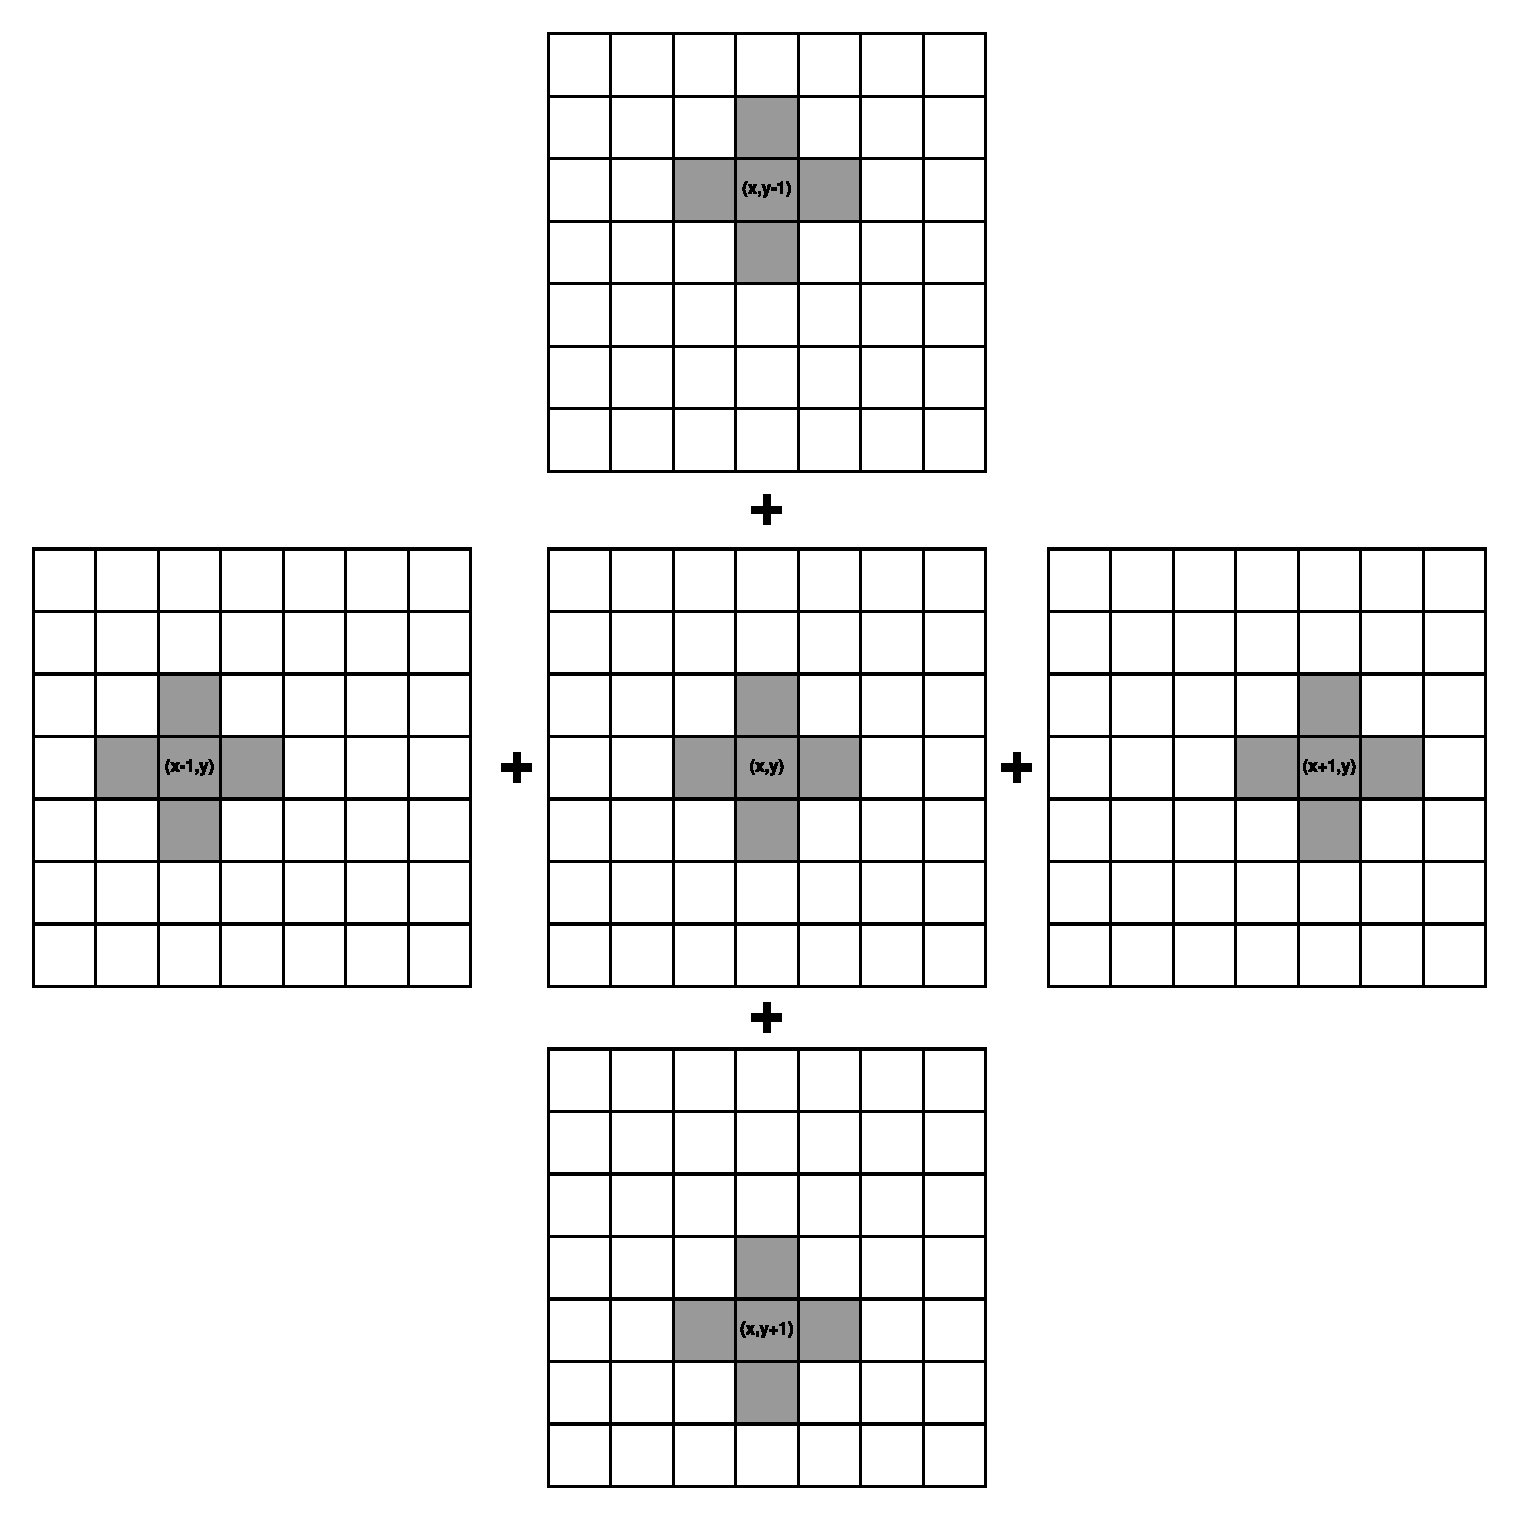
\includegraphics[width=\textwidth]{sources/max_manhattan/images/neighborhoodDP1_1}
        \caption[]{Manahtann neighborhoods of size $1$ for the cells:  $(x,y)$ (center), $(x+1,y)$ (right), $(x-1,y)$ (left), $(x,y-1)$ (top) and $(x,y+1)$ (down).}
        \label{fig:max_manhattan:neighborhoodDP1_1}
     \end{subfigure}
    
     \hfill
    
    \begin{subfigure}[t]{0.4\textwidth}
        \centering
        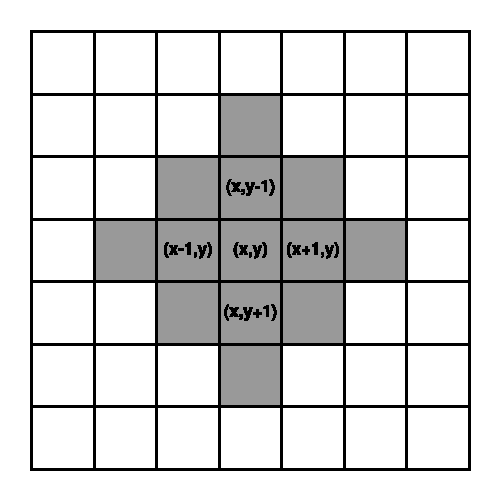
\includegraphics[width=\textwidth]{sources/max_manhattan/images/neighborhoodDP1_2}
        \caption[]{Neighborhood of size $2$ for the cell $(x,y)$ obtained by the union of the
        neighborhood depicted in Figure\ref{fig:max_manhattan:neighborhoodDP1_1}.}
        \label{fig:max_manhattan:neighborhoodDP1_2}
     \end{subfigure}
     \label{}
     \caption{}
\end{figure}

We can apply the same line of reasoning for finding the answer for $K=3$. Figure
\ref{fig:max_manhattan:neighborhoodDPK2_1} shows  the neighborhoods of size $2$ for the cells 
\begin{itemize*}
    \item $(x,y)$
    \item $(x+1,y)$
    \item $(x-1,y)$
    \item $(x,y-1)$
    \item $(x,y+1)$ \end{itemize*} and and Figure \ref{fig:max_manhattan:neighborhoodDPK2_2} shows
the neighborhood of size $3$ for the cell $(x,y)$. Also in this case the latter can be obtained by
the union of all the cells in Figure \ref{fig:max_manhattan:neighborhoodDPK2_1} and therefore, if we
have the answer for all the sub-problems where $K=2$ we can obtain the answer for the sub-problems
where $K=3$ without having to scan the entirety of the neighborhood of size $3$ for $(x,y)$. We only
have to find the maximum among $5$ elements instead of having to look into $25$ cells. This idea can
be generalized and its formalization is shown in Equation \ref{eq:max_manhattan:dpformula}. The
formula is saying that we can obtain the answer for $K=0$ trivially by simply returning the value of
the cell $(i,j)$. For $K>0$, we only have to return the max among the neighboring north,south, west
and east cells of $(i,j)$ for the same subproblem where at $K-1$.

\hspace{-0.5in}
\vspace{-0.051in}
\begin{equation}
    \begin{cases}
        S(0,i,j) = I[i][j] \\
        S(K,i,j) = \max \Big [ S(K-1,i,j), S(K-1,i+1,j),\;S(K-1,i-1,j),\;S(K-1,i,j+1),\;S(K-1,i,j-1) \Big ] \\
     \end{cases}
    \label{eq:max_manhattan:dpformula}
\end{equation}

\begin{figure}
    \vspace*{-0.5in}
    %\hspace*{-0.5in}
    \centering
    
    \begin{subfigure}[t]{1.0\textwidth}
        \centering
        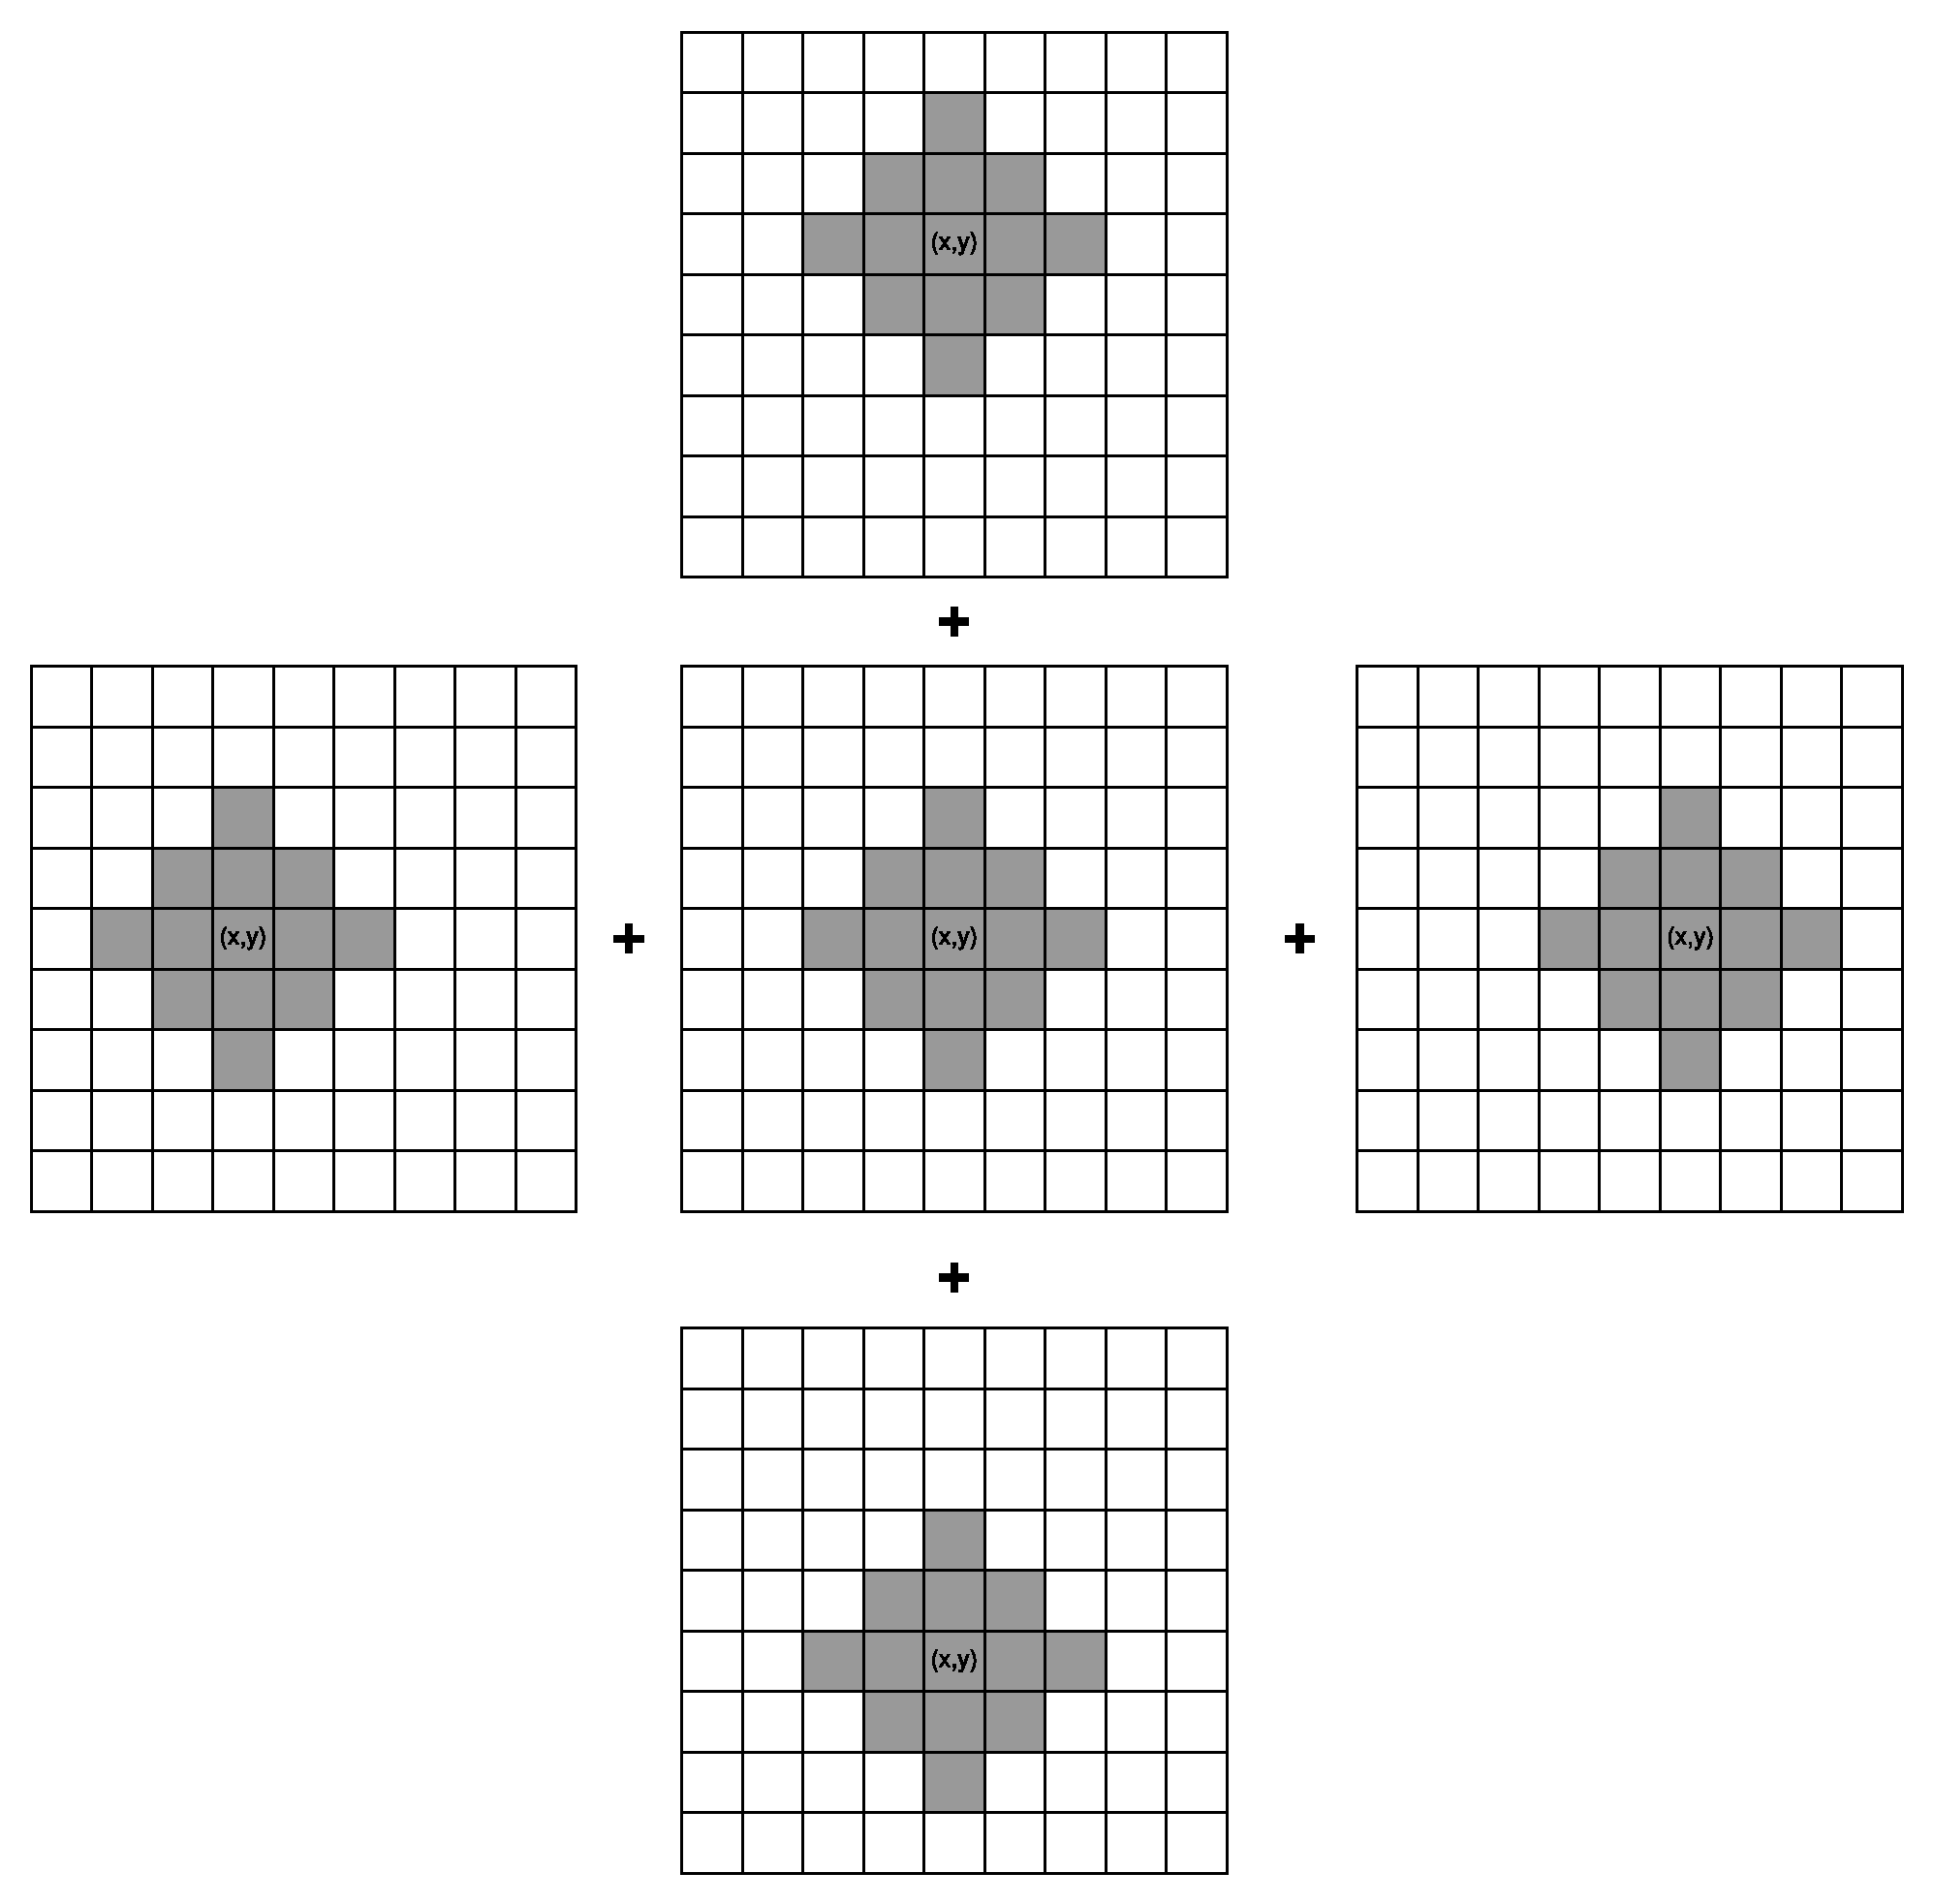
\includegraphics[width=\textwidth]{sources/max_manhattan/images/neighborhoodDPK2_1}
        \caption[]{Manahtann neighborhoods of size $1$ for the cells: $(x,y)$ (center), $(x+1,y)$ (right), $(x-1,y)$ (left), $(x,y-1)$ (top) and $(x,y+1)$ (down).}
        \label{fig:max_manhattan:neighborhoodDPK2_1}
    \end{subfigure}
    
    \hfill
    
    \begin{subfigure}[t]{0.4\textwidth}
        \centering
        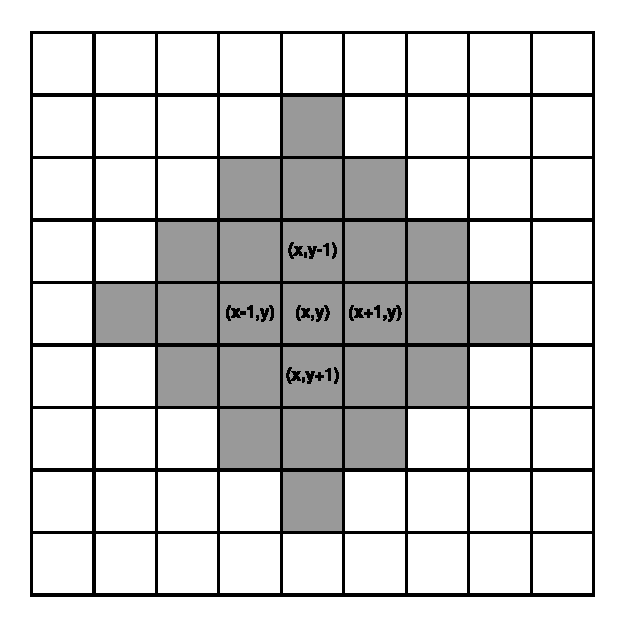
\includegraphics[width=\textwidth]{sources/max_manhattan/images/neighborhoodDPK2_2}
        \caption[]{Neighborhood of size $3$ for the cell $(x,y)$ obtained by the union of the
        neighborhood depicted in Figure\ref{fig:max_manhattan:neighborhoodDPK2_1}.}
        \label{fig:max_manhattan:neighborhoodDPK2_2}
     \end{subfigure}
     \label{}
     \caption{}
\end{figure}


As for all dynamic programming problem, we have two ways to write the solution:
\begin{enumerate}
    \item top-down, where we use memoization to avoid making duplicate work
    \item bottom-up, where we solve subproblem in an ordered manner, from the simplest one to the
    hardest.
\end{enumerate}

\subsubsection{Top-down}
\label{sec:max_manhattan:topdown}
The top-down approach is possibly the easiest to write as we can  translate $S(K,i,j)$ (see Equation
\ref{eq:max_manhattan:dpformula}) into a C++ recursive function, and we can use memoization (in the
form of a cache of size $K\times n\times m$) to store intermediate values of $S$ and avoid duplicate
work. Listing \ref{list:max_manhattan:dp_topdown} shows an implementation of this approach where
such a cache is implemented via a hashmap, which maps the arguments of $S$, all triplets $(K,i,j)$,
to integers. Notice that the function \inline{hash\_combine} and the functor \inline{TupleHash} are
the machinery that makes us use tuples of type \inline{std::tuple<int,int,int>} as keys in the Cache
(which has type \inline{std::unordered_map}). \inline{TupleHash} uses \inline{hash\_combine} to
calculate the hash value for a given \inline{std::tuple<int,int,int>}. The main driver function is
named \inline{max\_manhattan\_matrix\_k\_DP\_topdown} and the sole purpouse is to create the
memoization cache and then to call the C++ equivalent of function $S$ (see Equation
\ref{eq:max_manhattan:dpformula}): \inline{max\_manhattan\_matrix\_k\_DP\_topdown\_helper}. The
latter is a recursive function that takes as input
\begin{enumerate*}
    \item the original input matrix $I$ (which is never modified and it is only passed along as a
    reference),
    \item $K$, the max distance at which we search for the max value in $I$ ,
    \item \inline{cell}, which contains the coordinate of the cell for which we are finding and
    answer, and finally
    \item the memoization cache where we store the answers for a given $K$ and \inline{cell}.
\end{enumerate*}

The first thing we do is to unpack the cell into two separate variables representing the row and the
column of a cell: $i,j$. If the coordinate of the cell are outside the boundaries of $I$, then there
is no answer for such cell and we return the smallest possible int. Moreover if $K=0$, as per
Equation \ref{eq:max_manhattan:dpformula}, the answer is the value of the cell $(i,j)$ When we have
already calculate the solution to this very problem (i.e. for the same values of $K,i,j$) then we
simply return the memoized value. In all the other cases, we have to do the actual work and perform
the recursive calls to get the answer for the subproblems for the neighboring cells at the previous
value of $K$:
\begin{itemize}
    \item \inline{max\_manhattan\_matrix\_k\_DP\_topdown\_helper(K-1,i-1,j)}
    \item \inline{max\_manhattan\_matrix\_k\_DP\_topdown\_helper(K-1,i+1,j)}
    \item \inline{max\_manhattan\_matrix\_k\_DP\_topdown\_helper(K-1,i,j+1)}
    \item \inline{max\_manhattan\_matrix\_k\_DP\_topdown\_helper(K-1,i,j-1)} \end{itemize}.

The time and space complexity of this approach is $O(nmK)$. The proof is quite simple and it boils
down to the following facts:
\begin{enumerate}
    \item there are exactly $n\times m \times K$ different unique ways we can call the recursive
    function.
    \item each function call is memoized. This means that redundant work is avoided, therefore we do
    not do the work for a recursive call that has been already executed fully.
\end{enumerate}
Clearly each entry in the memoization cache costs $4$ integers for a total of $O(nmK)$.

\lstinputlisting[language=c++, caption={DP top-down solution to the problem of finding the max cell within the manhattan neighborhood of size $K$.},label=list:max_manhattan:dp_topdown]{sources/max_manhattan/max_manhattan_solution2.cpp}



\subsubsection{Bottom-up}
If we pay closer attention to Equation \ref{eq:max_manhattan:dpformula} or, equivalently to the
top-down implementation in Listing \ref{list:max_manhattan:dp_topdown} we immediately notice that in
order to calculate all the values of $S(K,i,j)$ for a given $K$ we only need the values of $S$ for
$K-1$. Because we know that the solution to the sub-problems where $K=0$, we can immediately solve
all the problems where $K=1$. At this point the values for the sub-problems where $K=0$ are not
needed anymore and we can throw them away and use that space to store the solution for the
sub-problems where $K=1$. Now that we have the solution for all sub-problems where $K=1$, we can proceed and calculate the
solutions for $K=2$. We apply the same line of reasoning to the rest of the sub-problems
 until we reach the value of $K$ we need.

The bottom-up approach is built on that idea and works by iteratively computing the answers for
sub-problems where $K-1$ before moving on calculating the answer for the sub-problems for the next
value of $K$. This can be implemented by using two matrices of the same size of $I$:
\begin{itemize}
    \item $M_{K-1}$: storing the values of the sub-problems for the previous value of $K$ we are
    trying to compute during this step.
    \item $M_{K}$ which is the space where we write the answers for the sub-problems we calculate
    during this step.
\end{itemize}
When $M_{K}$ is full and ready, it can be copied into $M_{K-1}$ and continue to process the next
value of $K$. In other words, $M_{K}$ is a working space where the solutions to the sub-problems for
the current $K$ are stored, and $M_{K-1}$ contains all the answers for the sub-problems necessary to
calculate the answers at the step.

The computation of a value of $M_{K}$ uses the same idea the top-down approach uses: the value of
to $M_K[i][j]$ is the maximum  among the following five values: 
\begin{enumerate*}
    \item $M_{K-1}[i][j]$
    \item $M_{K-1}[i+1][j]$
    \item $M_{K-1}[i-1][j]$
    \item $M_{K-1}[i][j+1]$
    \item $M_{K-1}[i][j-1]$
\end{enumerate*}

Notice that at any time, all the space we need is the space for storing the solution for the
sub-problems for two different values of $K$. This translated into a significant reduction in  space
complexity w.r.t. the top-down approach described in Section \ref{sec:max_manhattan:topdown} which
is in this approach $O(nm)$.

Listing \ref{list:max_manhattan:dp_bottomup} shows an implementation of this idea. Notice that in
the actual code, $M_{K-1}$ and $M_{K}$ are the variables \inline{previous} and \inline{current},
respectively. 
\lstinputlisting[language=c++, caption={DP bottom-down solution to the problem of finding the max cell within the manhattan neighborhood of size $K$.},label=list:max_manhattan:dp_bottomup]{sources/max_manhattan/max_manhattan_solution3.cpp}

%This problem can be solved easily using dynamic programming. DP recurrence: dp[k][i][j] = ans. for
%kth manhattan distance for element (i,j) dp[k+1][i][j] = max(dp[k][i-1][j], dp[k][i+1][j],
%dp[k][i][j-1], dp[k][i][j+1], dp[k][i][j] ) Recurrence is easy to get once you draw the figure.